%!TEX program = lualatex

\PassOptionsToPackage{french}{babel}
\PassOptionsToPackage{french}{translator}
\PassOptionsToPackage{table,svgnames}{xcolor}
\documentclass[aspectratio=169,11pt]{beamer}

%----------------------------------------
% Packages
%----------------------------------------
\usepackage{etoolbox}
\usepackage{ifxetex}
\usepackage{ifluatex}
\usepackage[T1]{fontenc}
\ifboolexpr{bool{xetex} or bool{luatex}}{%
	\usepackage{fontspec}
}{%
	\usepackage[utf8]{inputenc}
}
\usepackage{babel}
\usepackage{translator}
\usepackage{lmodern}
\usepackage{hyperref}
\usepackage{xcolor}
\usepackage{listings}
\usepackage{amsmath}
\usepackage{amssymb}
\usepackage{mathrsfs}
\usepackage{blkarray}
\usepackage{dsfont}
\usepackage{braket}
\usepackage{array}
\usepackage{tabularx}
\usepackage{multirow}
\usepackage{booktabs}
\usepackage[justification=centering]{caption}
\usepackage{float}
\usepackage[mode=tex]{standalone}
\usepackage{pgf}
\usepackage{pgfplots}
\pgfplotsset{compat=newest}
\usepackage{tikz}
\usepackage{tikzpeople}
\usepackage[backend=bibtex,bibstyle=ieee,citestyle=numeric-comp]{biblatex}

%----------------------------------------
% Theme
%----------------------------------------

\usetheme[nofirafonts,numbering=progressbar]{focus}
% \usetheme[numbering=fullbar]{focus}
% \usetheme[numbering=none]{focus}
% \definecolor{main}{RGB}{92, 138, 168}
% \definecolor{background}{RGB}{240, 247, 255}

% remove navigation symbols.
\beamertemplatenavigationsymbolsempty{}

%\setbeamercovered{transparent}

%----------------------------------------
% Informations
%----------------------------------------

\title{Set Cover Problem}
\subtitle{}
\author{Benoît Cortier\\Maxime Pinard}
\institute[UQAC]{Université du Québec à Chicoutimi\\555 Boulevard de l'Université, Chicoutimi, QC G7H 2B1}
\date[18/04/2019]{18 Avril 2019}

%\keywords{}
\subject{Set Cover Problem}
%\logo{\includegraphics[width=0.12\textwidth]{logos/UQAC}}

%----------------------------------------
% Bibliography
%----------------------------------------

\bibliography{../references}
\nocite{*}

%----------------------------------------
% Figures
%----------------------------------------

% Common file
\usetikzlibrary{shapes}
\usetikzlibrary{arrows.meta}
\usetikzlibrary{calc}
\usetikzlibrary{positioning}
\usetikzlibrary{angles}
\usetikzlibrary{quotes}
\usetikzlibrary{decorations}

\definecolor{bg_color}{RGB}{250,250,229}
\definecolor{Cblue}{RGB}{38,75,150}
\definecolor{Cgreen}{RGB}{39,179,118}
\definecolor{Cdarkgreen}{RGB}{0,111,60}
\definecolor{Corange}{RGB}{249,167,62}
\definecolor{Cred}{RGB}{191,33,47}

\colorlet{good}{green!90!black}
\colorlet{average}{Corange}
\colorlet{bad}{Cred}


% Figures folder
\graphicspath{{../figures/}}

%----------------------------------------
% Tables
%----------------------------------------

% Common file
\newcolumntype{L}[1]{>{\raggedright\let\newline\\\arraybackslash\hspace{0pt}}m{#1}}
\newcolumntype{C}[1]{>{\centering\let\newline\\\arraybackslash\hspace{0pt}}m{#1}}
\newcolumntype{R}[1]{>{\raggedleft\let\newline\\\arraybackslash\hspace{0pt}}m{#1}}
\newcolumntype{Y}{>{\centering\arraybackslash}X}


%----------------------------------------
% Plots
%----------------------------------------

\pgfplotsset{
	table/search path={../plots},
}

%----------------------------------------
% Document
%----------------------------------------
\begin{document}
	\begin{frame}
		\titlepage
	\end{frame}
	% \begin{frame}{Sommaire}
	% 	\tableofcontents
	% \end{frame}

	%% définition du problème

	\begin{frame}
		\frametitle{Définition du « Set Cover Problem » (SCP)}
		\begin{block}{Notation}
			\begin{itemize}
				\item \(U = \{u_1, u_2, u_3, \dots, u_m\}\), ensemble univers composé de \(m\) points
				\item \(S = \{s_1, s_2, \dots, s_n\}\), famille de \(n\) sous-ensembles de \(U\)
			\end{itemize}
		\end{block}
		\begin{block}<2->{Objectif}
			\begin{itemize}
				\item[\alert{\(\blacktriangleright\)}] Trouver une sous-famille de \(S\) la plus petite possible permettant de couvrir chaque élément de \(U\) au moins une fois.
				\item \(e\) est couvert par un sous-ensemble \(A\) si \(e \in A\).
			\end{itemize}
		\end{block}
		% \begin{block}{Solution}
		% 	Vecteur \(n\)-dimensionnel \(x = \left(x_j\right)\) avec
		% 	\[\forall j \in N,\ x_j = \left\{
		% 		\begin{array}{ll}
		% 			1 & \text{si } u_i \text{ fait parti de la solution}\\
		% 			0 & \text{sinon}
		% 		\end{array}
		% 	\right.\]
		% \end{block}
	\end{frame}

	\begin{frame}
		\frametitle{Exemple minimal: SCP}
		\centering
		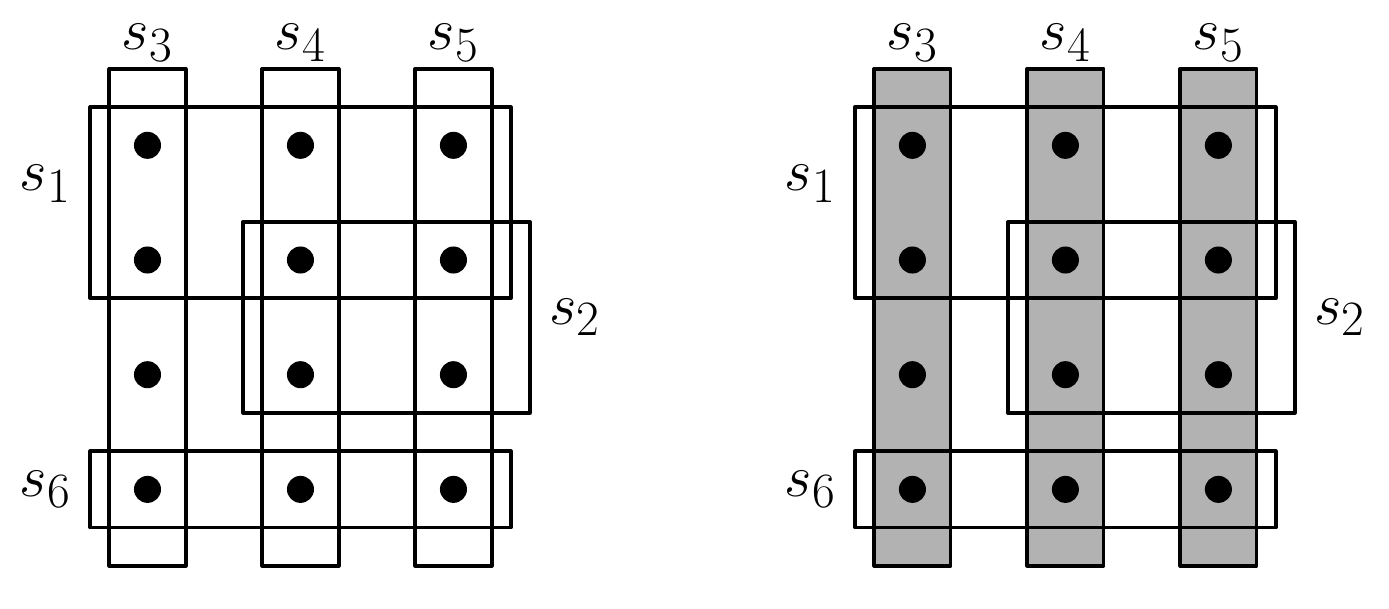
\includegraphics[width=0.85\linewidth]{scp_example}%
	\end{frame}

	\begin{frame}
		\frametitle{Définition du « Weighted Set Cover Problem » (WSCP)}
		\begin{block}{Notation}
			On pose \(M = \{1,\ldots,m\}\) et \(N = \{1,\ldots,n\}\)
			\begin{itemize}
				\item \(U = \{u_1, u_2, u_3, \dots, u_m\}\), ensemble univers composé de \(m\) points
				\item \(S = \{s_1, s_2, \dots, s_n\}\), famille de \(n\) sous-ensembles de \(U\)
				\item \(c = \left(c_j\right)\), vecteur coût \(n\)-dimensionnel avec \(\forall j \in N\), \(c_j\) le coût du sous-ensemble \(j\)
			\end{itemize}
		\end{block}
		\begin{block}<2->{Matrice d'incidence}
			\(A = \left(a_{i,j}\right)\) de taille \(m \times n\) avec
			\[\forall i \in M,\ \forall j \in N,\ a_{i,j} = \left\{
				\begin{array}{ll}
					1 & \text{si } u_i \in s_j \\
					0 & \text{sinon}
				\end{array}
			\right.\]
			\(a_{i,j} = 1\) signifiant donc que le point \(i\) est couvert par le sous-ensemble \(j\)
		\end{block}
	\end{frame}
	\begin{frame}
		\frametitle{Exemple minimal: WSC}
		\[
		\begin{blockarray}{ccccccccc}
			& s_1 & s_2 & s_3 & s_4 & s_5 & s_6 & s_7 \\
			\begin{block}{c(ccccccc)c}
				   & 0 & 1 & 1 & 0 & 0 & 0 & 1 & u_1\\
				   & 0 & 0 & 1 & 0 & 1 & 1 & 0 & u_2\\
				A= & 1 & 1 & 0 & 1 & 0 & 1 & 0 & u_3\\
				   & 0 & 0 & 0 & 0 & 1 & 1 & 1 & u_3\\
				   & 1 & 0 & 1 & 0 & 0 & 0 & 1 & u_4\\
			\end{block}
			\\
			\begin{block}{c(ccccccc)c}
				c = & 3 & 1 & 2 & 4 & 1 & 2 & 1 &\\
			\end{block}
		\end{blockarray}
		\]
	\end{frame}

	\begin{frame}
		\frametitle{Définition du « Weighted Set Cover Problem » (WSCP)}
		\begin{block}{Objectif}
			\begin{itemize}
				\item[\alert{\(\blacktriangleright\)}] Trouver une sous-famille de \(S\) avec \alert{le plus petit coût} possible permettant de couvrir chaque élément de \(U\) au moins une fois.
				\item \(e\) est couvert par un sous-ensemble \(A\) si \(e \in A\).
			\end{itemize}
		\end{block}
		\begin{block}<2->{Solution}
			Vecteur \(n\)-dimensionnel \(x = \left(x_j\right)\) avec
			\[\forall j \in N,\ x_j = \left\{
				\begin{array}{ll}
					1 & \text{si } u_i \text{ fait parti de la solution}\\
					0 & \text{sinon}
				\end{array}
			\right.\]
			La solution a comme coût \(\sum_{j \in N}{c_i x_i}\) et est valide si
			\(\forall i \in M\ ,\sum_{j \in N}{a_{ij}x_i} \ge 1\)
		\end{block}
	\end{frame}

	%% exemple minimal

	\begin{frame}
		\frametitle{Exemple minimal: WSC}
		\[
		\begin{blockarray}{ccccccccc}
			& s_1 & s_2 & s_3 & s_4 & s_5 & s_6 & s_7 \\
			\begin{block}{c(ccccccc)c}
				    & 0 & 1 & 1 & 0 & 0 & 0 & 1 & u_1\\
				    & 0 & 0 & 1 & 0 & 1 & 1 & 0 & u_2\\
				A = & 1 & 1 & 0 & 1 & 0 & 1 & 0 & u_3\\
				    & 0 & 0 & 0 & 0 & 1 & 1 & 1 & u_3\\
				    & 1 & 0 & 1 & 0 & 0 & 0 & 1 & u_4\\
			\end{block}
			\\
			\begin{block}{c(ccccccc)c}
				c = & 3 & 1 & 2 & 4 & 1 & 2 & 1 &\\
			\end{block}
			\\
			\begin{block}{c(ccccccc)c}
				x = & 0 & 1 & 1 & 0 & 0 & 0 & 1 &\\
			\end{block}
		\end{blockarray}
		\]
	\end{frame}

	%% complexité NP-complétude

	\begin{frame}
		\frametitle{Complexité}
		\begin{block}{}
			\begin{itemize}
				\item l'un des 21 problèmes NP-complets de \citeauthor{Karp1972}~\cite{Karp1972}.
				\item NP-complet au sens fort~\cite{garey2002computers}.
			\end{itemize}
		\end{block}
		\begin{exampleblock}{}
			\fullcite{Karp1972}
		\end{exampleblock}
	\end{frame}

	\begin{frame}
		\frametitle{Complexité}
		\centering
		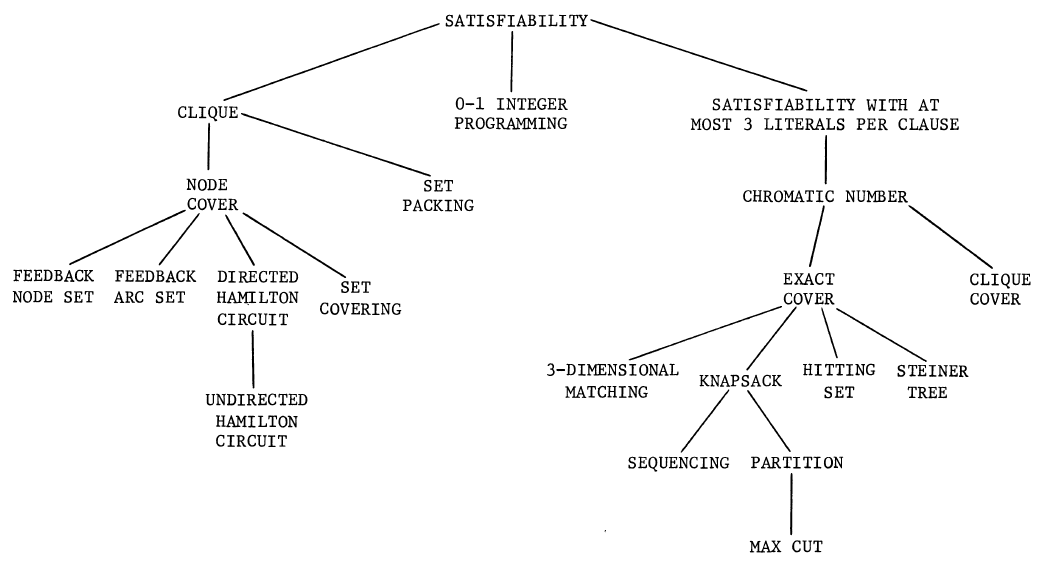
\includegraphics[width=0.9\linewidth]{karp_reduction_tree}%
	\end{frame}

	\begin{frame}
		\frametitle{Complexité}
		\begin{block}{Théorème de Cook-Levin}
			Le problème de satisfiabilité d'une formule de la logique propositionnelle (SAT), est NP-complet.
		\end{block}
		\begin{exampleblock}{}
			\fullcite{Cook1971}
		\end{exampleblock}
	\end{frame}

	%% état de l'art

	\begin{frame}
		\frametitle{État de l'art}
		\begin{block}{Méthodes exactes}
			\begin{itemize}
				\item le plus efficace: méthodes branch-and-bound en calculant les bornes inférieures à l'aide d'une relaxation du problème en programmation linéaire.~\cite{caprara2000algorithms}
				\item Algorithme de \citeauthor{Beasley1987}: le nœud racine utilise la solution du programme linéaire relaxé, puis les bornes inférieures sont calculées à l'aide de la relaxation lagrangienne.~\cite{Beasley1987}
			\end{itemize}
		\end{block}
	\end{frame}
	\begin{frame}
		\frametitle{État de l'art}
		\begin{block}{Méthodes approchées voraces}
			\begin{itemize}
				\item L'algorithme vorace standard de \citeauthor{Johnson:1973:AAC:800125.804034} pour le problème de couverture d'ensemble non pondéré. L'algorithme prend simplement le sous-ensemble qui couvre le plus d'éléments à chaque étape jusqu'à obtenir une solution valide. Complexité en \(O(mn)\).~\cite{Johnson:1973:AAC:800125.804034}
				\item \citeauthor{Goldschmidt:1993:MGH:177276.177287}: méthode où l'on applique des
					algorithmes approchés et exacts.
					On utilise l'algorithme vorace de Johnson jusqu'à obtenir une taille maximale de 2.
					On peut trouver la solution optimale pour une taille maximale de 2 en un temps linéaire.~\cite{Goldschmidt:1993:MGH:177276.177287}
			\end{itemize}
		\end{block}
	\end{frame}

	\begin{frame}
		\frametitle{État de l'art}
		\begin{block}{Méthode approchée métaheuristique: \citeauthor{Beasley1990}}
			À chaque itération d'un gradient: un ensemble \(S\) est initialisé avec les sous-ensembles sélectionnés par la solution de la relaxation lagrangienne. Puis, pour chaque point non couvert par \(S\), le sous ensemble avec le coût original le plus faible est ajouté à \(S\). Pour finir, les différents sous-ensembles de \(S\) sont considérés par ordre de coût original décroissant et on enlève le sous-ensemble \(j\) si \(S \backslash \{j\}\) est toujours une solution valide.~\cite{Beasley1990}
		\end{block}
	\end{frame}

	\begin{frame}
		\frametitle{État de l'art}
		\begin{block}{Méthode approchée métaheuristique: \citeauthor{jacobs1995lsh}}
			Approche basée sur le recuit simulé.~\cite{jacobs1995lsh}
			\begin{itemize}
				\item Solution initiale \(S\) est générée par un algorithme vorace.
				\item On execute un certain nombre d'itérations de recuit simulé:
				on choisi un sous-ensemble dans \(S\) aléatoirement
				et on l'enlève, puis on complète de manière vorace de manière à obtenir une autre solution valide \(S'\).
				\item On décide si on garde ou non \(S'\).
			\end{itemize}
		\end{block}
	\end{frame}

	\begin{frame}
		\frametitle{État de l'art}
		\begin{block}{Méthode approchée métaheuristique: \citeauthor{Afif1995}}
			Méthode basée sur l'algorithme du flot de Ford-Fulkerson \(\rightarrow\) temps polynomial. Il s'agit d'effectuer une transformation du problème en un graphe de flot à résoudre par une variante de l'algorithme.~\cite{Afif1995}
		\end{block}
	\end{frame}

	%% représentation du problème

	\begin{frame}
		\centering TODO
	\end{frame}

	%% Instances de problèmes

	\begin{frame}
		\frametitle{OR-Library}
		\centering\resizebox{0.85\linewidth}{!}{%!TEX root = ../set_cover_problem.tex
\begin{tabular}{*{5}{C{65pt}}}
	\toprule
	Groupe d'instances & Nombre de lignes (\(m\)) [points] & Nombre de colonnes (\(n\)) [sous-ensembles] & densité (\%) & Nombre d'instances du groupe\\
	\midrule
	4 & 200 & 1000 & 2 & 10\\
	5 & 200 & 2000 & 2 & 10\\
	6 & 200 & 1000 & 5 & 5\\
	A & 300 & 3000 & 2 & 5\\
	B & 300 & 3000 & 5 & 5\\
	C & 400 & 4000 & 2 & 5\\
	D & 400 & 4000 & 5 & 5\\
	E & 500 & 5000 & 10 & 5\\
	F & 500 & 5000 & 20 & 5\\
	G & 1000 & 10000 & 2 & 5\\
	H & 1000 & 10000 & 5 & 5\\
	\bottomrule
\end{tabular}}
	\end{frame}
	\begin{frame}
		\frametitle{OR-Library}
		\hfill%
		\begin{minipage}{0.24\linewidth}
			\resizebox{\linewidth}{!}{%!TEX root = ../set_cover_problem.tex
\begin{tabular}{*{2}{C{65pt}}}
	\toprule
	Problem number & Optimal solution value\\
	\midrule
	4.1 & 429\\
	4.2 & 512\\
	4.3 & 516\\
	4.4 & 494\\
	4.5 & 512\\
	4.6 & 560\\
	4.7 & 430\\
	4.8 & 792\\
	4.9 & 641\\
	4.10 & 514\\
	\midrule
	5.1 & 253\\
	5.2 & 302\\
	5.3 & 226\\
	5.4 & 242\\
	5.5 & 211\\
	5.6 & 213\\
	5.7 & 293\\
	5.8 & 288\\
	5.9 & 279\\
	5.10 & 265\\
	\bottomrule
\end{tabular}}%
		\end{minipage}
		\hfill%
		\begin{minipage}{0.24\linewidth}
			\resizebox{\linewidth}{!}{%!TEX root = ../set_cover_problem.tex
\begin{tabular}{*{2}{C{65pt}}}
	\toprule
	Problem number & Optimal solution value\\
	\midrule
	A.1 & 253\\
	A.2 & 252\\
	A.3 & 232\\
	A.4 & 234\\
	A.5 & 236\\
	\midrule
	B.1 & 69\\
	B.2 & 76\\
	B.3 & 80\\
	B.4 & 79\\
	B.5 & 72\\
	\midrule
	C.1 & 227\\
	C.2 & 219\\
	C.3 & 243\\
	C.4 & 219\\
	C.5 & 215\\
	\midrule
	D.1 & 60\\
	D.2 & 66\\
	D.3 & 72\\
	D.4 & 62\\
	D.5 & 61\\
	\bottomrule
\end{tabular}}%
		\end{minipage}
		\hfill\hspace{0pt}
	\end{frame}
	\begin{frame}
		\frametitle{Problèmes générés}
		\hfill%
		\begin{minipage}{0.21\linewidth}
			\resizebox{\linewidth}{!}{%!TEX root = ../set_cover_problem.tex
\begin{tabular}{*{2}{C{65pt}}}
	\toprule
	Problem size & Optimal solution value\\
	\midrule
	&\\
	2 & 65\\
	3 & 63\\
	4 & 165\\
	5 & 183\\
	6 & 220\\
	7 & 224\\
	8 & 230\\
	9 & 163\\
	10 & 287\\
	11 & 253\\
	12 & 223\\
	13 & 345\\
	14 & 336\\
	15 & 391\\
	16 & 356\\
	17 & 249\\
	18 & 243\\
	19 & 264\\
	20 & 288\\
	21 & 390\\
	22 & 300\\
	23 & 234\\
	24 & 244\\
	25 & 274\\
	\bottomrule
\end{tabular}}%
		\end{minipage}
		\hfill%
		\begin{minipage}{0.21\linewidth}
			\resizebox{\linewidth}{!}{%!TEX root = ../set_cover_problem.tex
\begin{tabular}{*{2}{C{65pt}}}
	\toprule
	Problem size & Optimal solution value\\
	\midrule
	26 & 460\\
	27 & 336\\
	28 & 315\\
	29 & 253\\
	30 & 256\\
	31 & 327\\
	32 & 409\\
	33 & 401\\
	34 & 334\\
	35 & 185\\
	36 & 411\\
	37 & 310\\
	38 & 247\\
	39 & 247\\
	40 & 358\\
	41 & 398\\
	42 & 368\\
	43 & 507\\
	44 & 360\\
	45 & 305\\
	46 & 263\\
	47 & 278\\
	48 & 214\\
	49 & 270\\
	50 & -\\
	\bottomrule
\end{tabular}}%
		\end{minipage}
		\hfill%
		\begin{minipage}{0.21\linewidth}
			\resizebox{\linewidth}{!}{%!TEX root = ../set_cover_problem.tex
\begin{tabular}{*{2}{C{65pt}}}
	\toprule
	Problem size & Optimal solution value\\
	\midrule
	51 & 317\\
	52 & 185\\
	53 & 275\\
	54 & 261\\
	55 & 302\\
	56 & 261\\
	57 & 279\\
	58 & -\\
	59 & -\\
	60 & 309\\
	61 & 129\\
	62 & 260\\
	63 & -\\
	64 & 290\\
	65 & 200\\
	66 & -\\
	67 & 195\\
	68 & 231\\
	69 & -\\
	70 & 225\\
	71 & -\\
	72 & -\\
	73 & 141\\
	74 & -\\
	75 & -\\
	\bottomrule
\end{tabular}}%
		\end{minipage}
		\hfill%
		\begin{minipage}{0.21\linewidth}
			\resizebox{\linewidth}{!}{%!TEX root = ../set_cover_problem.tex
\begin{tabular}{*{2}{C{65pt}}}
	\toprule
	Problem size & Optimal solution value\\
	\midrule
	76 & -\\
	77 & 226\\
	78 & 186\\
	79 & 166\\
	80 & 276\\
	81 & -\\
	82 & -\\
	83 & -\\
	84 & -\\
	85 & -\\
	86 & -\\
	87 & -\\
	88 & -\\
	89 & 219\\
	90 & -\\
	91 & -\\
	92 & 222\\
	93 & 150\\
	94 & -\\
	95 & -\\
	96 & -\\
	97 & 202\\
	98 & -\\
	99 & -\\
	100 & 193\\
	\bottomrule
\end{tabular}}%
		\end{minipage}
		\hfill\hspace{0pt}
	\end{frame}

	%% méthodes exactes
	\section{Méthodes exactes}

	\begin{frame}
		\frametitle{Exemple: plot}
		\centering
		\begin{tikzpicture}
	\begin{axis}[
		width=\linewidth,
		height=0.5\linewidth,
		xlabel={taille du bitset (nombre de bits)},
		ylabel={RAM utilisée (Go)},
		xmin=0, xmax=40,
		ymin=0, ymax=9,
		legend style={
			cells={
				anchor=west
			},
			legend pos=north west,
		},
	]
		\addplot[smooth,color=blue,mark=square*] table{g1_ram.data};
		\addlegendentry{G1: ram expensive generator}
		\addplot[smooth,color=red,mark=*] table{g2_ram.data};
		\addlegendentry{G2: cpu expensive generator}
		\addplot[smooth,color=cyan,mark=triangle*] table{g3_ram.data};
		\addlegendentry{G3: counter generator}
	\end{axis}
\end{tikzpicture}%%
	\end{frame}

	%% méthodes approchées
	\section{Méthodes approchées}

	\begin{frame}
		\frametitle{Méthodes voraces implémentées (non optimales)}
		\begin{block}{Méthode vorace non pondérée}
			\begin{itemize}
				\item Greedy classique de \citeauthor{Johnson:1973:AAC:800125.804034}: sélection de l'ensemble qui couvre le plus de nouveaux points successivement.
				\item[\alert{\(\blacktriangleright\)}]<2-> Problème \emph{A.1} (optimal: \(253\)), on obtient la solution de coût \alert{\(1444\)}.
			\end{itemize}
		\end{block}
		\begin{block}<3->{Méthode vorace pondérée}
			\begin{itemize}
				\item Greedy basé sur celui de \citeauthor{Johnson:1973:AAC:800125.804034}: on utilise le rapport \(\frac{n}{c}\) avec
					\begin{itemize}
						\item \(n\) le nombre de nouveaux points couverts,
						\item et \(c\) le coût du sous-ensemble.
					\end{itemize}
				\item[\alert{\(\blacktriangleright\)}]<4-> Problème \emph{A.1} (optimal: \(253\)), on obtient cette fois une solution de coût \alert{\(288\)}.
			\end{itemize}
		\end{block}
	\end{frame}

	\begin{frame}
		%\frametitle{Comparaison des méthodes voraces}
		\centering
		\begin{tikzpicture}
	\begin{axis}[
		width=\linewidth,
		height=0.6\linewidth,
		xlabel={Taille du problème (nombre de sous-ensembles)},
		ylabel={Ratio de différence à l'optimale},
		xmin=0, xmax=101,
		ymin=0, ymax=3.1,
		legend style={
			cells={
				anchor=west
			},
			legend pos=north west,
		},
	]
		\addplot[unbounded coords=jump,smooth,color=blue,mark=square*] table{data/ugreedy_diff.data};
		\addlegendentry{Unweighted Greedy}
		\addplot[unbounded coords=jump,smooth,color=red,mark=*] table{data/wgreedy_diff.data};
		\addlegendentry{Weighted Greedy}
	\end{axis}
\end{tikzpicture}%

	\end{frame}

	\begin{frame}
		\frametitle{Recuit simulé}
		\begin{itemize}
			\item Recuit simulé standard (vu en cours)
			\item On applique un opérateur de voisinage à chaque itération
			\item Si cela améliore la solution, on conserve la solution, sinon on on accepte avec une
				probalité \(e^{\frac{-\Delta}{T}}\) avec \(\Delta\) la différence de coût
				entre la solution courante et la nouvelle solution et \(T\) la température courante.
			\item Nous faisons varier la température uniformément entre deux bornes au fil des itérations.
		\end{itemize}
	\end{frame}

	\begin{frame}
		\frametitle{Algorithme génétique}
		\begin{itemize}
			\item Sélection par rang
			\item Recherche locale à l'aide du recuit simulé
			\item Opérateur de croisement: résoudre le problème de façon vorace à l'aide de la méthode vorace pondérée
				sur les sous-ensembles choisis par les deux solutions à croiser uniquement.
		\end{itemize}
	\end{frame}

	\begin{frame}
		\frametitle{Algorithme génétique: procédure}
		\begin{itemize}
			\item On commence par générer une population \(P\) de \(n\) individus aléatoirement.
			\item À chaque itération (ou génération):
				\begin{itemize}
					\item On trie les individus par coût décroissant. L'indice d'un individu correspond alors à son rang.
					\item On supprime les individus on doublon pour favoriser l'exploration. On note \(D\) le nombre de doublons supprimés.
					\item On créer \(n' = n \times t_r\) nouveaux individus à partir de deux parents à chaque fois.
						Les deux parents sont sélectionnés selon leur rang. On applique un opérateur de croisement
						pour obtenir une troisième solution. Cette solution a une probabilité \(t_l\) de subir une
						recherche locale par recuit simulé avec les paramètres \(r_{tmp}\) et \(r_{fin}\) et une probabilité
						\(t_m\) de subir une mutation par opérateur de voisinage.
					\item Les \(n'\) nouveaux individus remplacement les \(n' - D\) pire individus de la génération précédente.
				\end{itemize}
			\item On élémine des sous-ensembles de la meilleure solution trouvée en lançant la procédure vorace pondérée limitée
				aux sous-ensembles choisis par la solution.
			\item On retourne cette solution.
		\end{itemize}
	\end{frame}

	%% comparaison avec les méthodes approchées

	\begin{frame}
		\frametitle{Évaluation des méthodes présentées}
		\begin{block}{Instances d'OR-Library utilisées}
			\begin{itemize}
				\item avec solution optimale: A.1, B.1, C.1., D.1, 4.1, 5.1
				\item sans solution optimale: 6.1.
			\end{itemize}
		\end{block}
		\begin{block}<2->{Ajustement des paramètres par optimisation de boîte noire}
			\begin{itemize}
				\item Algorithme de Mesh Adaptive Directed Search avec le logiciel NOMAD\footnote{{https://sourceforge.net/projects/nomad-bb-opt/}}
				\item Fonctionne autant avec des boîtes noires déterministes qu'avec des boite non-déterministes.
			\end{itemize}
		\end{block}
	\end{frame}
	\begin{frame}
		\frametitle{Évaluation des méthodes présentées}
		\begin{block}{Configuration}
			\begin{itemize}
				\item Algorithme génétique:
					\begin{itemize}
						\item 60 évaluations de boîte noire maximum
						\item l'évaluation dure une minute: on effectue autant de générations que possible durant le temps imparti
					\end{itemize}
				\item Recuit simulé:
					\begin{itemize}
						\item 20 évaluations de boîte noire maximum
						\item \(50\,000\,000\) d'itérations (3 minutes)
						\item solution de départ générée aléatoirement
					\end{itemize}
			\end{itemize}
		\end{block}
	\end{frame}

	\begin{frame}
		\frametitle{Coût des solutions obtenues}
		\centering
		%!TEX root = ../set_cover_problem.tex
\begin{tabular}{*{5}{c}}
	\toprule
	Problème & Optimal & Weighted Greedy & Recuit simulé  & Algorithme génétique \\
	\midrule
	A.1      & 253     & 288 (13.8\%)    & 276 (9.09\%)    & 257 (1.58\%) \\
	\midrule
	B.1      & 69      & 77 (11.6\%)     & 80  (15.9\%)   & 70 (1.45\%) \\
	\midrule
	C.1      & 227     & 258 (13.7\%)    & 277 (22.0\%)   & 232 (2.20\%) \\
	\midrule
	D.1      & 60      & 74 (23.3\%)     & 71 (18.3\%)    & 62 (3.33\%) \\
	\midrule
	4.1      & 429     & 463 (7.93\%)    & 434 (1.17\%)   & 433 (0.93\%) \\
	\midrule
	5.1      & 253     & 289 (14.2\%)    & 286 (13.0\%)   & 260 (2.77\%) \\
	\midrule
	6.1      & -       & 159             & 143            & 138 \\
	\bottomrule
\end{tabular}


	\end{frame}

	\section*{Questions?}
		\begin{frame}[focus]
			Questions?
		\end{frame}
	\appendix
		\begin{frame}[t,allowframebreaks]
			\frametitle{Références}
			\printbibliography[heading=bibintoc]{}
		\end{frame}
\end{document}
